% Lecture Template for ME3050-001-002-Tristan Hill - Spring 2020
% Dynamics Modeling and Controls
% Laplace Transforms - Module 10 - Topic 1

% I am finally converting my stuff to BEAMER

% Document settings

%\documentclass{beamer}                  % for presentation ?
\documentclass[handout]{beamer}  % for handout ?
\usepackage{beamerthemesplit}
\usepackage{amsmath}
\usepackage{listings}
\usepackage{multicol}
\usepackage{framed}

\beamertemplateballitem

\definecolor{TTUpurple}{rgb}{0.3098, 0.1607, 0.5176} % TTU Purple (primary)
\definecolor{TTUgold}{rgb}{1.0000, 0.8666, 0.0000} % TTU Gold (primary)

\setbeamercolor{palette primary}{bg=TTUpurple,fg=TTUgold}
\setbeamercolor{palette secondary}{bg=black,fg=TTUgold}
\setbeamercolor{palette tertiary}{bg=black,fg=TTUpurple}
\setbeamercolor{palette quaternary}{bg=TTUgold,fg=black}
\setbeamercolor{structure}{fg=TTUpurple} % itemize, enumerate, etc
\setbeamercolor{section in toc}{fg=TTUpurple} % TOC sections

%\usefonttheme{professionalfonts}

\newcommand{\Lagr}{\mathcal{L}} % lagrangian

\newcommand{\hspcu}{\underline{\hspace{20mm}}} % large horizontal space w underline
\newcommand{\vspccc}{\vspace{6mm}\\} % large vertical space
\newcommand{\vspcc}{\vspace{4mm}\\}   % medium vertical space
\newcommand{\vspc}{\vspace{2mm}\\}     % small vertical space

\newcommand{\hspcccc}{\hspace{10mm}} % large horizontal space
\newcommand{\hspccc}{\hspace{6mm}} % large horizontal space
\newcommand{\hspcc}{\hspace{4mm}}   % medium horizontal space
\newcommand{\hspc}{\hspace{2mm}}     % small horizontal space

\newsavebox{\mybox} % custom box

\newcommand{\MNUM}{10\hspace{2mm}} % Module number
\newcommand{\TNUM}{1\hspace{2mm}} % Topic number 
\newcommand{\moduletitle}{The Laplace Transform} % Titles and Stuff
\newcommand{\topictitle}{Definition of the Laplace Transform} 

\newcommand{\sectiontitleI}{An Integral Transform} % More Titles and Stuff
\newcommand{\sectiontitleII}{Laplace Transform of A Derivative}
\newcommand{\sectiontitleIII}{Properties of an Integral}
\newcommand{\sectiontitleIV}{Table of Transform Pairs}

\author{ME3050 - Dynamics Modeling and Controls}
\title{Module \MNUM - \moduletitle}
\date{Mechanical Engineering\vspc Tennessee Technological University}

\begin{document}

\lstset{language=MATLAB,basicstyle=\ttfamily\small,showstringspaces=false}

\frame{\titlepage \center\begin{framed}\Large \textbf{Topic \TNUM - \topictitle}\end{framed} \vspace{5mm}}

% Section 0 - Outline
\frame{
	
	\large \textbf{Topic \TNUM - \topictitle} \vspace{3mm}\\
	
	\begin{itemize}
	
		\item \sectiontitleI    \vspc % Section I
		\item \sectiontitleII 	\vspc % Section II
		\item \sectiontitleIII 	\vspc %Section III
		\item \sectiontitleIV 	\vspc %Section IV
	
	\end{itemize}

}


\section{\sectiontitleI}

\frame{ 
\frametitle{\sectiontitleI}

The Laplace Transform is an Integral Transform

Given a function $x(t)$ in the time domain where $t\geq0$, \\ the Laplace Transform is defined as follows: \\

\[ X(s)=\Lagr{\{x(t)\}}=\displaystyle\int_0^{\infty} x(t)e^{-st}dt \]\\

And its inverse is similarly defined as: \\

\[ \Lagr^{-1}{\{X(s)\}}=x(t) \]\\

The Laplace Domain variable $s$ is a complex number: \[ s=\sigma+j\omega \] 

}




\section{\sectiontitleII}
\frame{
\frametitle{\sectiontitleII}



It is useful to find the laplace transform of the derivative of a function: 
\[ \Lagr{\{\frac{d}{dt}(x(t))\} }=\Lagr{\{\dot{x}(t)\}} =s\Lagr{\{x(t)\} }-x(t=0) \]
\[ \hspace{52mm} =sX(s)-x(t=0) \]
\[ \hspace{52mm}\Lagr{\{ \dot{x} \left(t\right) \}} =sX(s)-x_0 \]

\[ \Lagr{\{\frac{d^2}{dt^2}(x(t))\} }=\Lagr{\{\ddot{x}(t)\}} = s^2\Lagr{\{x(t)\} }-sx(t=0)-\dot{x}(t=0) \]
\[ \hspace{52mm} = s^2X(s)-sx(t=0)-\dot{x}(t=0) \]
\[ \hspace{52mm} \Lagr{\{ \ddot{x} \left(t\right) \}}= s^2X(s)-sx_0-\dot{x}_0  \]


}

\section{\sectiontitleIII}
\frame{
\frametitle{\sectiontitleIII}

Also, remember that the transform inherits the properties of an integral.

\[ \int\left[ x(t)+y(t) \right]dt =\int x(t)dt + \int y(t)dt \]
\[ \int Kx(t)dt = K\int x(t)dt \hspcc (K \hspc is \hspc constant)\]

Therefore these properties can be used with the Laplace transform.
}

\section{\sectiontitleIV}
\frame{
\frametitle{\sectiontitleIV}

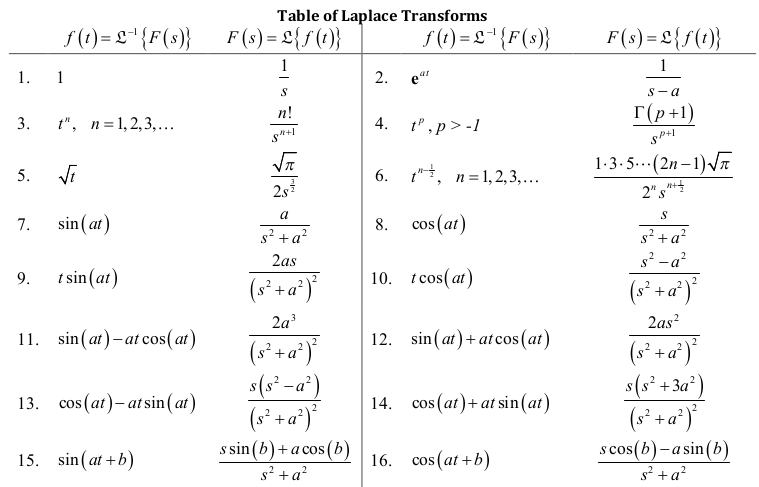
\includegraphics[scale=.35]{laplace_table_part1.png}


}

\frame{
\frametitle{\sectiontitleIV}

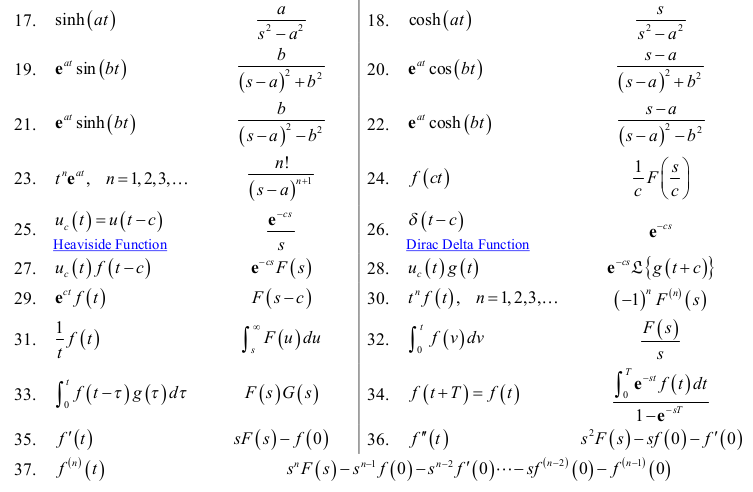
\includegraphics[scale=.35]{laplace_table_part2.png}


}



\end{document}

